
\documentclass[main.tex]{subfiles}

\begin{document}
\chapter{Experiment}
\label{ch:exp}
Följande avsnitt beskriver det experiment för att undersöka effektiviteten av filtrena. Vi beskriver först mätuppställningen, sedan utförda mätserier och till sist vilka parametrar som från modellanpassningen som jämförs och presenteras i resultatkapitlet.



\section{Mätuppställning}
Mätuppställningen är baserad på \figref{fig:matuppstallning}, men med våra filter på vardera sida om provlådan.

\begin{comment}
\begin{figure}
    \centering
    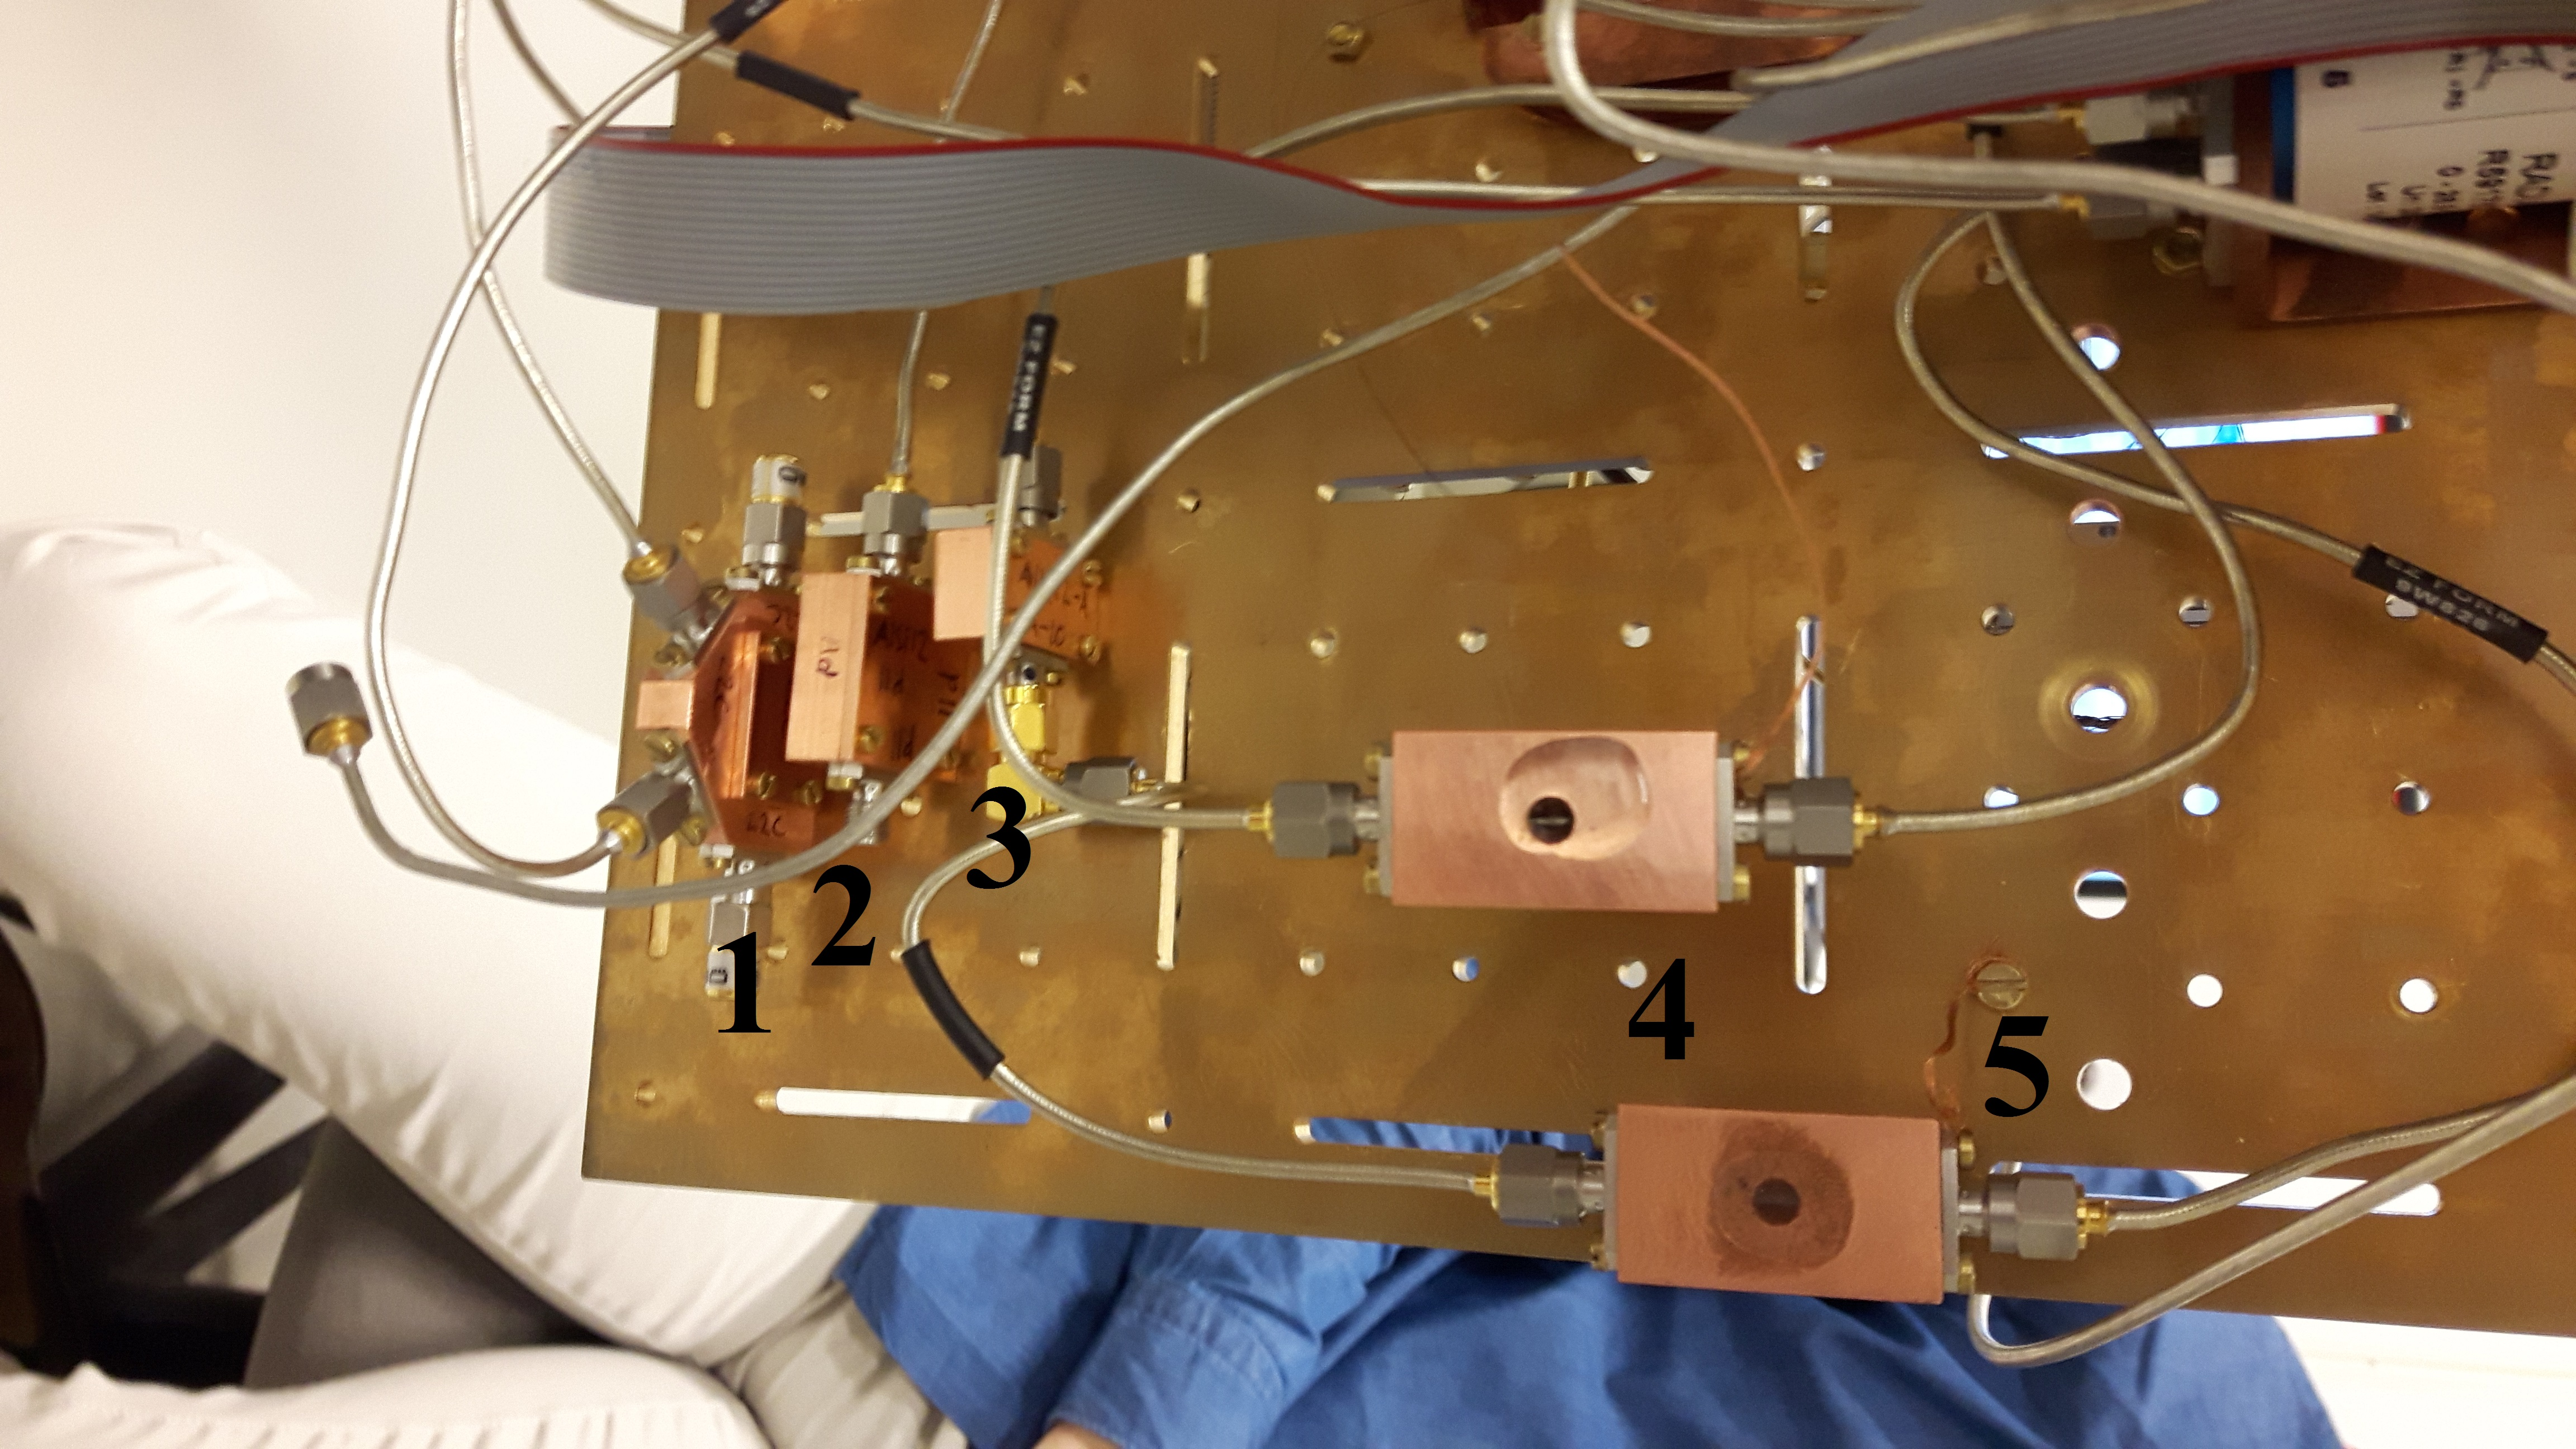
\includegraphics[scale=0.08,trim={35cm 8cm 20cm  20cm},clip]{figure/Experiment/siffroruppst.jpg}
    \caption{I figuren visas provlådorna AlSi12-22C (1), AlSi12-11d (2), och AlSi12-A (3). Till provlåda AlSi12-A är filtren med 1,895 cm respektive 1,825 cm frilagd ledare placerade (4). Filtren är kopplade till plattan med en koppartråd (5).}
    \label{fig:sifferupp}
\end{figure}
\end{comment}


\begin{comment}

\begin{figure}
    \centering
    \begin{tikzpicture}
        \node[anchor=south west,inner sep=0] (image) at (3,0) {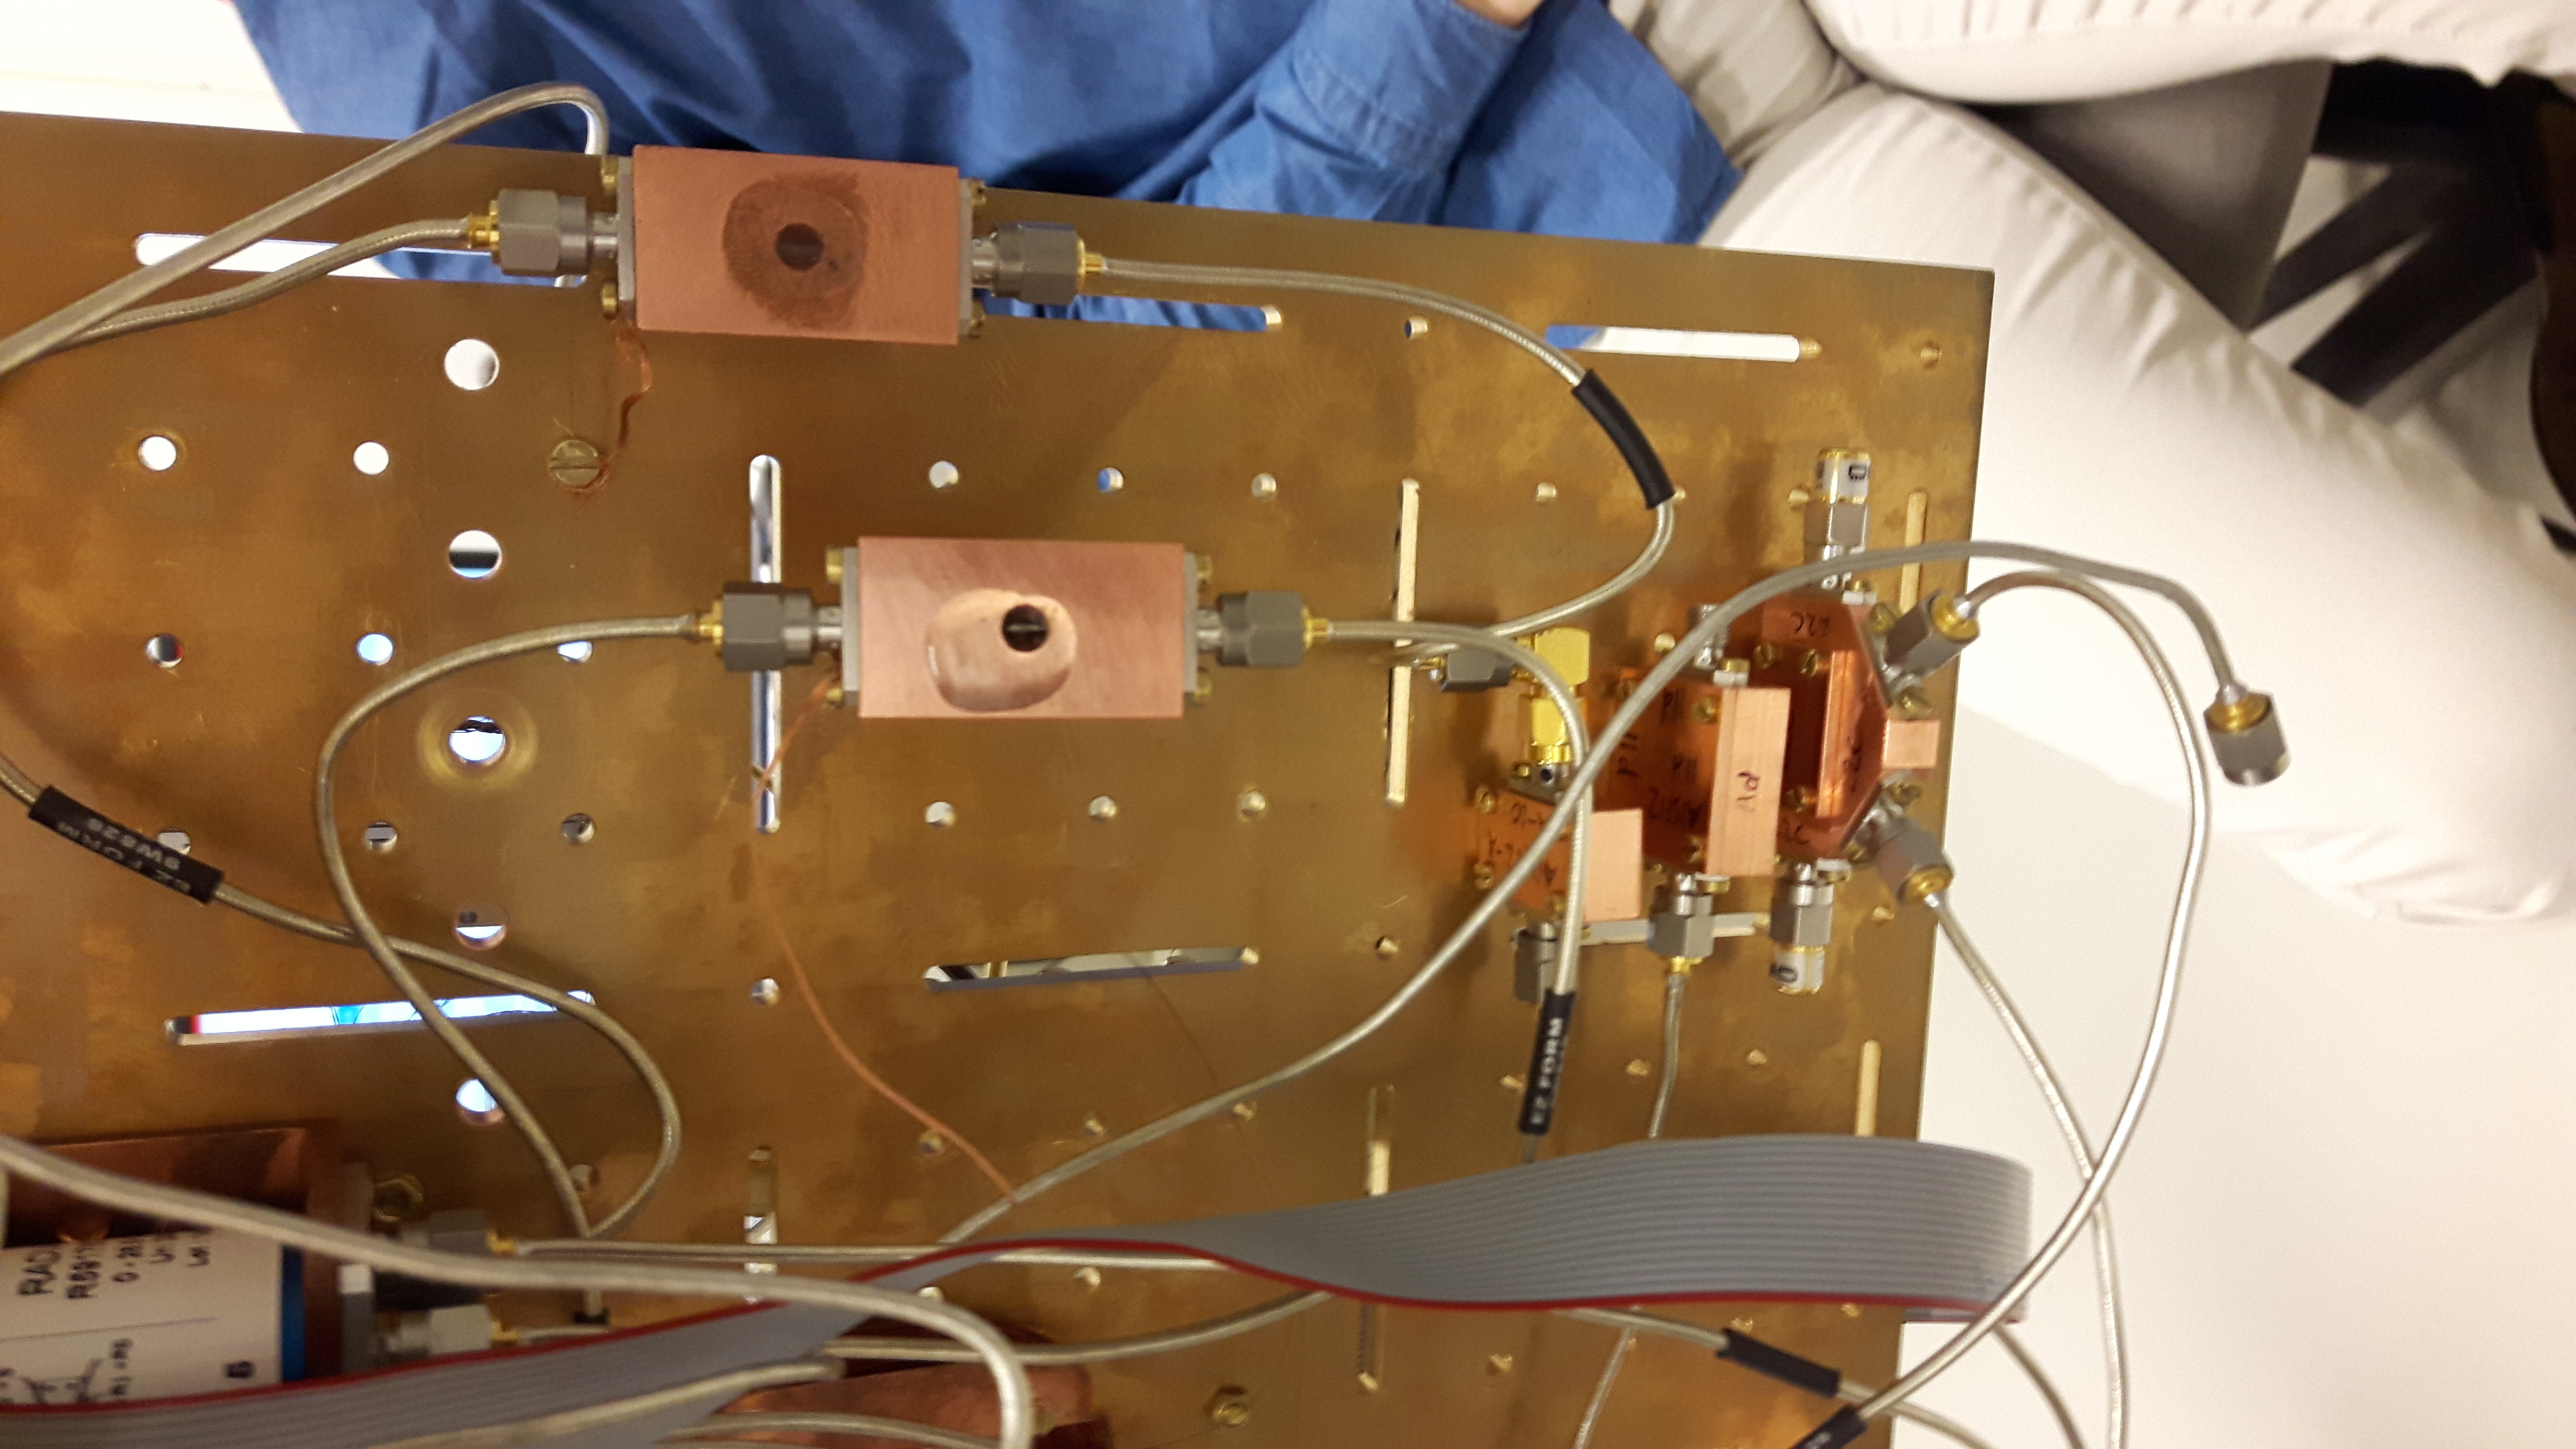
\includegraphics[width=0.1\textwidth,angle=180,trim=400 500 400 225,clip,width=0.75\linewidth]{figure/Experiment/uppstt.jpg}};
        \begin{scope}[x={(image.south east)},y={(image.north west)}]
        \node [anchor=west] at (0.3,0.4) {\Large\textbf 1};
        \node [anchor=west] at (0.34,0.4) {\Large\textbf 2};
        \node [anchor=west] at (0.4,0.45) {\Large\textbf 3};
        \node [anchor=west] at (0.65,0.3) {\Large\textbf 4};
        \node [anchor=west] at (0.8,0.35) {\Large\textbf 5};
        %\node [anchor=west] at (0.3,0.7) {\Large\textbf F};
        %\node [anchor=west] at (0.6,0.8) {\Large\textbf G};
        %\node [anchor=west] at (0.7,0.6) {\Large\textbf H};
        %\node [anchor=west] at (0.9,0.4) {\Large\textbf I};
        \end{scope}
    \end{tikzpicture}
    \caption{I figuren visas provlådorna AlSi12-22C (1), AlSi12-11d (2), och AlSi12-A (3). Till provlåda AlSi12-A är filtren med 1,895 cm respektive 1,825 cm frilagd ledare placerade (4). Filtren är kopplade till plattan med en koppartråd (5).}
    \label{fig:sifferupp}
\end{figure}


\end{comment}




Nio filter användes i mätningen, tre stycken med en frilagd ledare med en ungefärlig längd kring 1,85 cm (1,825 cm, 1,895 cm och 1,880 cm), tre stycken med en frilagd ledare med ungefärlig längd kring 2,5 cm (2,520 cm, 2,480 cm och 2,470 cm), och tre stycken med en frilagd ledare med ungefärlig längd kring 3,15 cm (3,145cm, 3,155cm och 3,150cm). Till varje provlåda placerades två filter med ungefär lika lång frilagd ledare, ett filter innan och ett efter, se figur \ref{fig:sifferupp} där enbart en av provlådorna har ett filter placerat före och efter sig. I tabell \ref{tab:filtertillbox} redovisas vilka filter som hörde till vilken provlåda. En koppartråd fästes även från varje filter till plattan som provlådorna var fästa vid. Detta gjordes för att uppnå termisk jämvikt eftersom värmeledningen i koaxial-kablarna kunde vara otillräcklig. % Tre filter, alla av olika längd, placerades även vid egna ingångar, för att utnyttja dessa som referenser vid låg temperatur. 

\begin{table}[h]
    \centering
        \caption{Provlåda med tillhörande filter. L$_i$ innebär längden på den frilagda ledaren i filtret placerat innan provlådan, L$_e$ innebär längden på dett}
    \label{tab:filtertillbox}
    \begin{tabular}{lccc}
    \toprule
        \textbf{Provlåda}  & Antal resonatorer & L$_i$ (cm) & L$_e$ (cm)\\
        \midrule
        AlSi12-A & 9 & 1.895 & 1.825\\
        AlSi12-22C & 6 & 3.145 & 3.150\\
        AlSi12-11d & 6 & 2.520 & 2.470\\
        \bottomrule
    \end{tabular}
\end{table}


\section{Mätserier}

\begin{figure}[h]
    \centering
    \setlength\figurewidth{0.45\textwidth}
    \setlength\figureheight{10em}
    % This file was created by matlab2tikz.
%
\definecolor{mycolor1}{rgb}{0.00000,0.44700,0.74100}%
%
\begin{tikzpicture}[%
trim axis left, trim axis right
]

\begin{axis}[%
width=\figurewidth,
height=\figureheight,
at={(0\figurewidth,0\figureheight)},
scale only axis,
xmin=-85,
xmax=-45,
xlabel style={font=\color{white!15!black}},
xlabel={Ineffekt (dBm)},
ymin=0,
ymax=250,
ylabel style={font=\color{white!15!black}},
ylabel={Medelvärdesbildningar},
axis background/.style={fill=white},
axis x line*=bottom,
axis y line*=left
]
\addplot [color=mycolor1, forget plot]
  table[row sep=crcr]{%
-83	240\\
-73	130\\
-63	35\\
-53	20\\
-48	15\\
};
\addplot [color=mycolor1, draw=none, mark=square, mark options={solid, mycolor1}, forget plot]
  table[row sep=crcr]{%
-83	240\\
-80.5	212.5\\
-78	185\\
-75.5	157.5\\
-73	130\\
-70.5	106.25\\
-68	82.5\\
-65.5	58.75\\
-63	35\\
-60.5	31.25\\
-58	27.5\\
-55.5	23.75\\
-53	20\\
-50.5	17.5\\
-48	15\\
};
\end{axis}
\end{tikzpicture}%
    \caption{Antal medelvärdesbildningar av VNA:n mot ineffekt}
    \label{fig:medel}
\end{figure}


En VNA av model Agilent E8364b användes för att svepa över ett frekvensspann mellan 2 och 8 GHz, detta för att finna de olika frekvenserna för resonatorerna. I provlåda A fanns nio resonatorer och i provlådorna C och d fanns sex stycken. Signalen från ett intervall på \unit[3]{MHz} kring centerfrekvenserna analyserades sedan där värdet på ineffekten varierades.


VNA:n svepte mellan en effekt på \unit[8]{dBm} och \unit[-27]{dBm} med en steglängd på \unit[2,5]{dBm}. För att nå ner till lägre effekter lades en dämpning till på input-kabeln. Först gjordes en mätning utan någon tillagd dämpning, denna behövde väldigt få medelvärdesbildningar eftersom bruset i förhållande till signalen är mycket lägre vid hög effekt. 

Vid andra svepet lades en dämpning på \unit[30]{dBm} genom att placera en \unit[20]{dBm} och en \unit[10]{dBm} dämpare på rad, då fick vi data för effekter mellan \unit[-22]{dBm} och \unit[-52]{dBm}. Här krävdes det fler medelvärdesbildningar än tidigare, vi använde oss av 32 stycken medelvärdesbildnignar. 

Vid tredje svepet placerades en dämpning på totalt \unit[56]{dBm} (20+30+6), den gick alltså mellan \unit[-44]{dBm} och \unit[-83]{dBm}, i detta fall behövdes det många fler medelvärdesbildningar eftersom vi arbetade med en sådan låg ineffekt att bruset var väldigt stort i relation till signalen. Antal medelvärdesbildningar som behövdes vid varje effekt visas i en graf i \figref{fig:medel}.

\subsection{Mätning 1, utan filter} 

I tabell \ref{tab:utanfil} visas centerfrekvenserna som användes i mätningarna.

\begin{table}[h]
    \centering
        \caption{Centerfrekvenser för resonatorerna i de olika provlådorna}
    \label{tab:utanfil}
    \begin{tabular}{lccccccccc}
    \toprule
        \textbf{Provlåda}  & \multicolumn{7}{c}{Centerfrekvenser (GHz)} \\
        \midrule
        AlSi12-A & 4,9527 & 5,0059 & 5,2182 & 5,6892 & 5,9586 & 6,2507 & 6,9457 & 7,3506 & 7,6232\\
        AlSi12-22C & 5,1535 & 5,3659 & 6,1322 & 6,4356 & 7,5693 & 7,8442 &\\
        AlSi12-11d & 4,8211 & 5,0110 & 5,7307 & 6,0239 & 7,0805  &  7,3207 & \\
        \bottomrule
    \end{tabular}
\end{table}



\subsection{Mätning 2, med filter}
På samma sätt som för mätningarna utan filter hittades centerfrekvenserna, dessa redovisas i tabell \ref{tab:centfil}.



\begin{comment}
\begin{table}[h]
\centering
\begin{tabular}{|c|c|c|c|}\hline
     Switch & Sample & Filter & Batch på filter (före,efter) \\\hline
     1 & A & Short & (1,3) \\\hline
     2 & d & Medium & (1,3) \\\hline
     3 & & Short & (2) \\\hline
     4 & C & Long & (1,3) \\\hline
     5 & & Long & (2) \\\hline
     6 & & Medium & (2) \\\hline
\end{tabular}
\end{table}

\end{comment}


\begin{comment}
\begin{table}[h]
    \centering
        \caption{Caption}
    \label{tab:centfil}
    \begin{tabular}{lccccccccc}
    \toprule
        \textbf{Provlåda}  & \multicolumn{7}{l}{Centerfrekvenser (GHz)} \\
        \midrule
        AlSi12-A & 4.9526 & 5.0061 & 5.2176 & 5.6892 & 5.9585 & 6.2505 & 6.9463 & 7.3508 & 7.6232\\
        AlSi12-22C & 5.1535 & 5.3655 & 6.1315 & 6.4357 & 7.5693 & 7.8443 &\\
        AlSi12-11d & 4.8218 & 5.0115 & 5.7314 & 6.0243 & 7.0812 & 7.3219 & \\
        \bottomrule
    \end{tabular}
\end{table}

\end{comment}

%\section{Parametrar från modellanpassningen}


\begin{comment}
\begin{figure}
    \begin{tikzpicture}
        \node[anchor=south west,inner sep=0] (image) at (0,0) {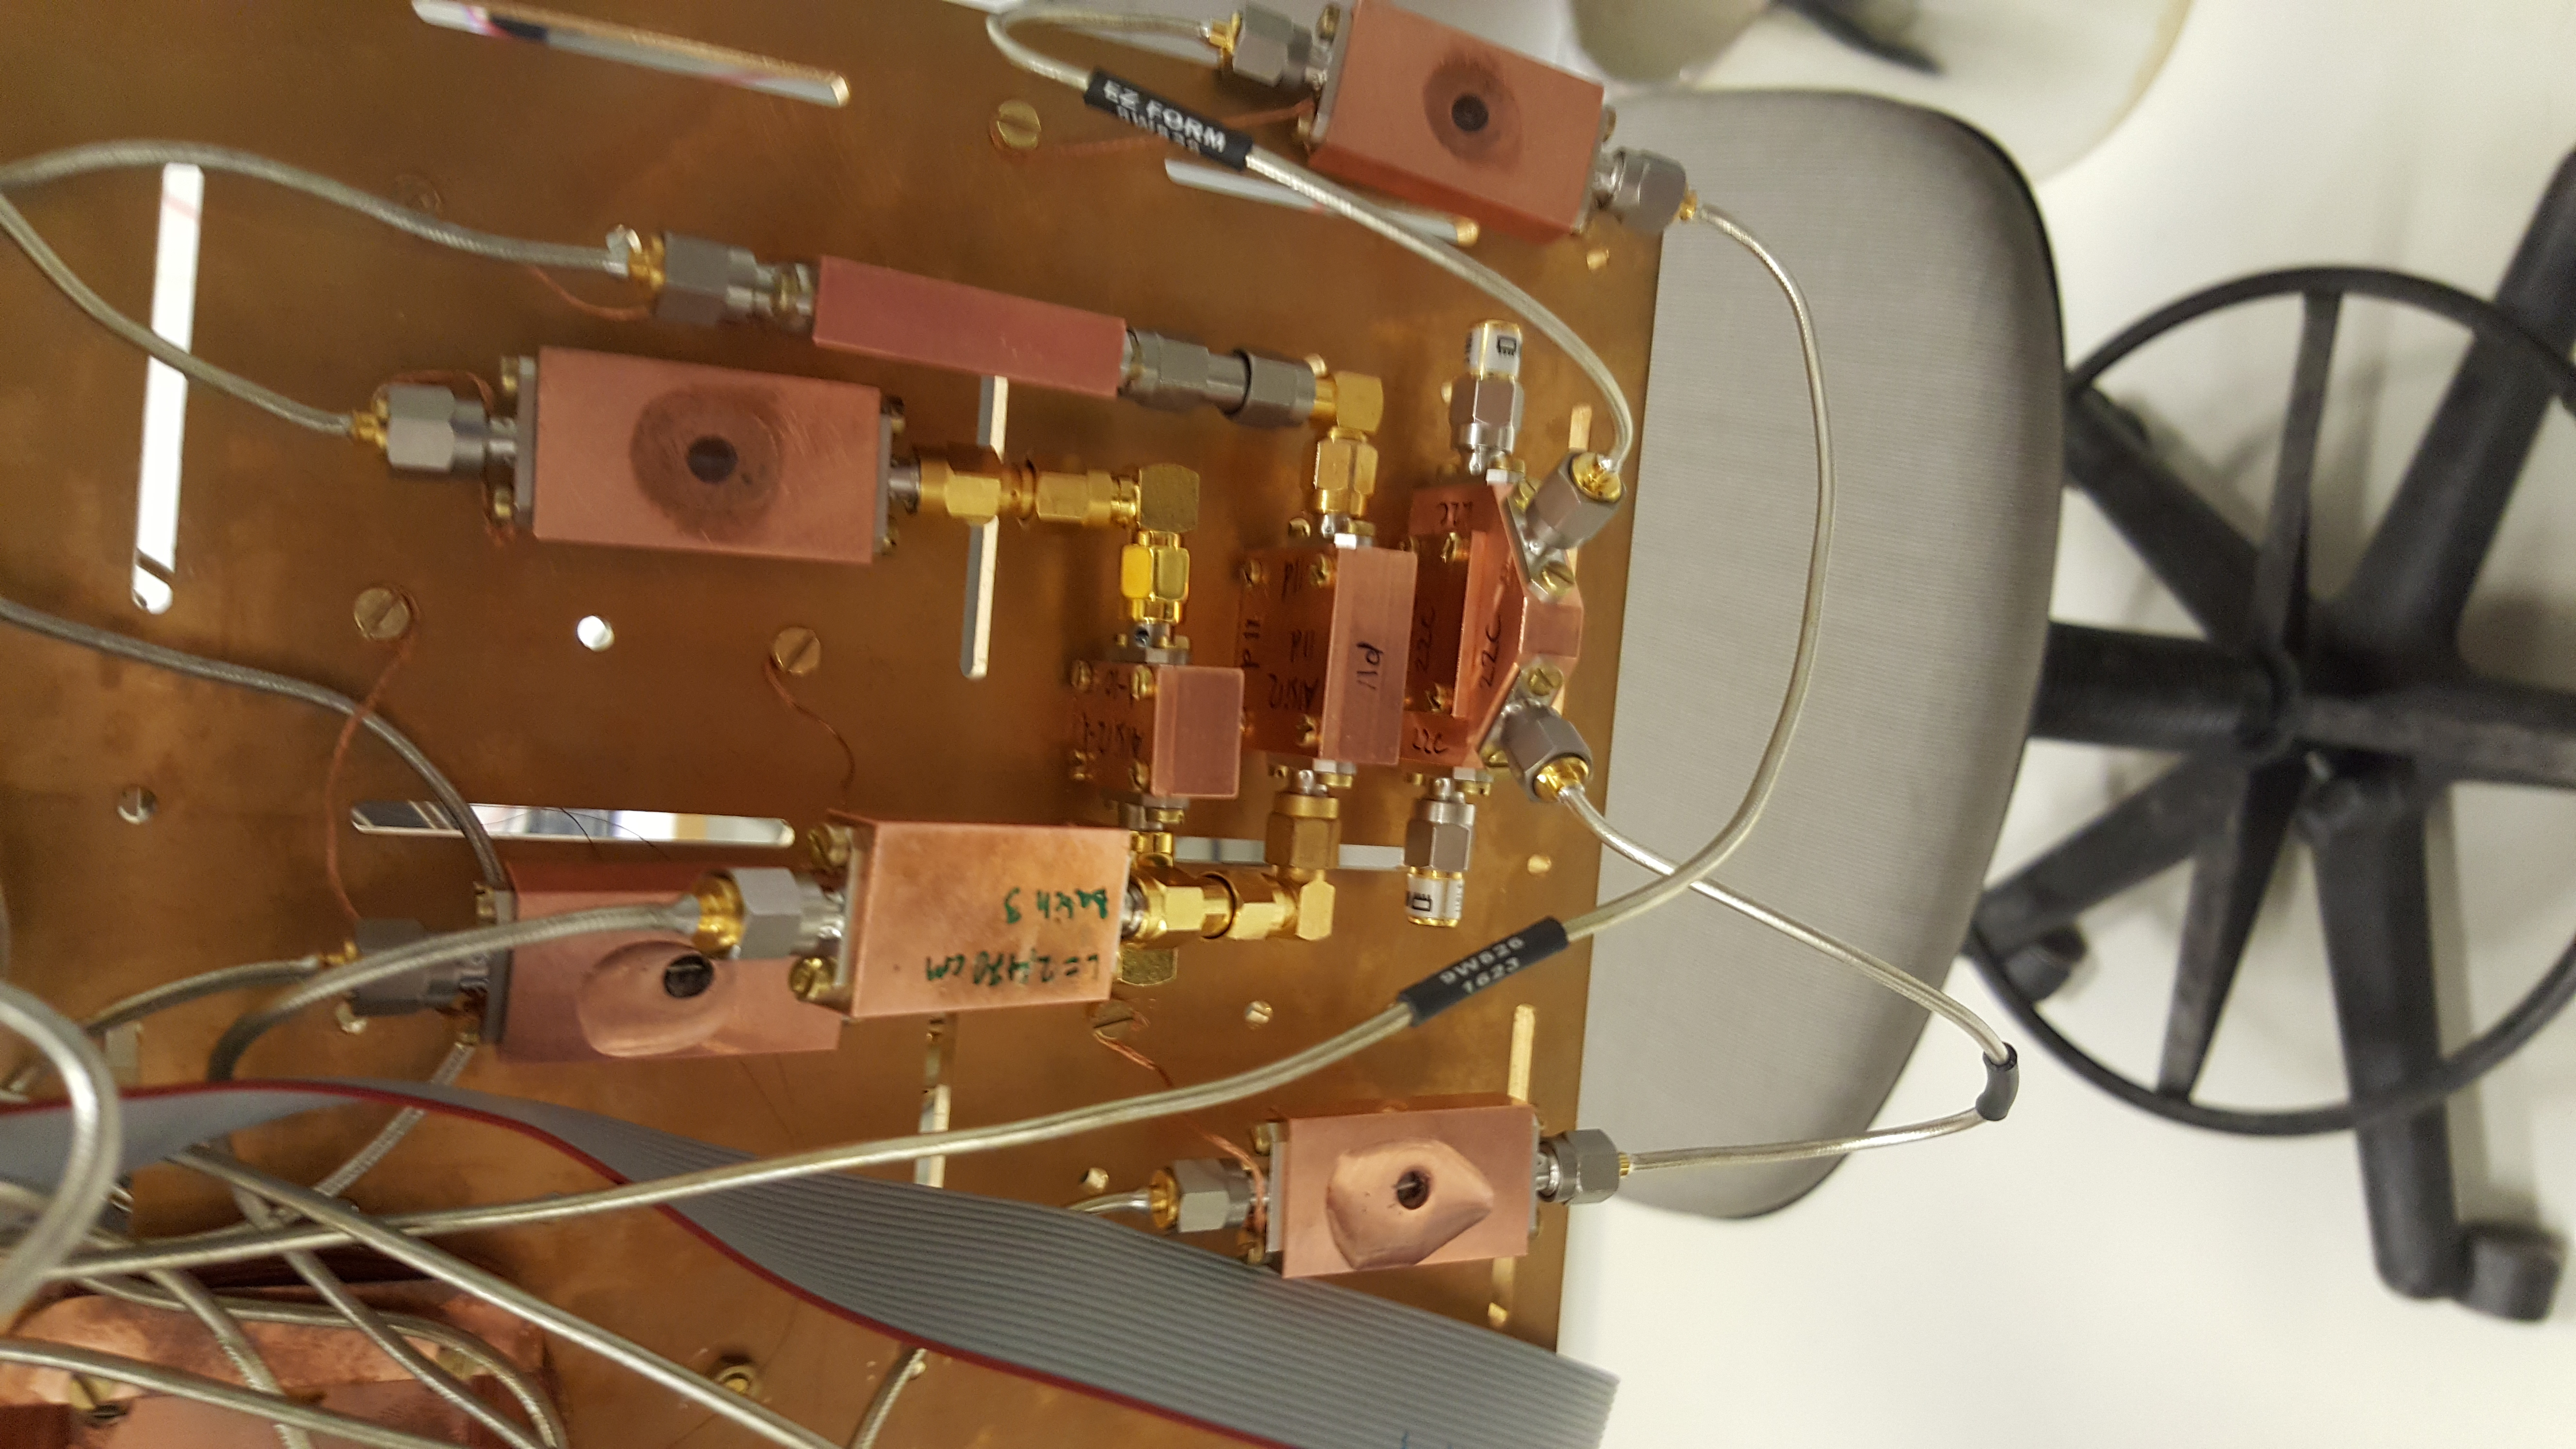
\includegraphics[width=0.75\textwidth,angle=-90,trim=1000 350 1700 0,clip,width=0.975\linewidth]{figure/Experiment/exp_ups.jpg}};
        \begin{scope}[x={(image.south east)},y={(image.north west)}]
        \node [anchor=west] at (0.5,0.5) {\Large\textbf A};
        \node [anchor=west] at (0.5,0.4) {\Large\textbf B};
        %\node [anchor=west] at (0.5,0.3) {\Large\textbf C};
        %\node [anchor=west] at (0,0.2) {\Large\textbf D};
        %\node [anchor=west] at (0.3,0.6) {\Large\textbf E};
        %\node [anchor=west] at (0.3,0.7) {\Large\textbf F};
        %\node [anchor=west] at (0.6,0.8) {\Large\textbf G};
        %\node [anchor=west] at (0.7,0.6) {\Large\textbf H};
        %\node [anchor=west] at (0.9,0.4) {\Large\textbf I};
        \end{scope}
    \end{tikzpicture}
    \caption{Temp caption}
    \label{}
\end{figure}

\end{comment}

\end{document}